\documentclass[10pt,twocolumn,letterpaper]{article}

\usepackage{cvpr}
\usepackage{times}
\usepackage{epsfig}
\usepackage{graphicx}
\usepackage{amsmath}
\usepackage{amssymb}

% Include other packages here, before hyperref.

% If you comment hyperref and then uncomment it, you should delete
% egpaper.aux before re-running latex.  (Or just hit 'q' on the first latex
% run, let it finish, and you should be clear).
\usepackage[pagebackref=true,breaklinks=true,letterpaper=true,colorlinks,bookmarks=false]{hyperref}

% \cvprfinalcopy % *** Uncomment this line for the final submission

\def\cvprPaperID{****} % *** Enter the CVPR Paper ID here
\def\httilde{\mbox{\tt\raisebox{-.5ex}{\symbol{126}}}}

% Pages are numbered in submission mode, and unnumbered in camera-ready
\ifcvprfinal\pagestyle{empty}\fi

\usepackage{color}

\newcommand{\matt}[1]{ \color{red} Matt: #1  \color{black}}
\newcommand{\aneesh}[1]{ \color{blue} Aneesh: #1  \color{black}}
\newcommand{\burak}[1]{ \color{green} Burak: #1  \color{black}}
\newcommand{\emmett}[1]{\color{violet} Emmett: #1  \color{black}}
\begin{document}


%%%%%%%%% TITLE
\title{Multiple Kernelized Correlation Filters based High Speed Target Following}

\author{Burak Uzkent\\
Rochester Institute of Technology\\
{\tt\small bxu2522@@rit.edu}
% For a paper whose authors are all at the same institution,
% omit the following lines up until the closing ``}''.
% Additional authors and addresses can be added with ``\and'',
% just like the second author.
% To save space, use either the email address or home page, not both
\and
YoungWoo Seo\\
Affiliation\\
{\tt\small yseo@autelrobotics.edu}
}

\maketitle
%\thispagestyle{empty}

%%%%%%%%% ABSTRACT
\begin{abstract}

\end{abstract}

%%%%%%%%% BODY TEXT
\section{Introduction}

A practical solution to target-following mode

\begin{itemize}
\item Introduction: Should talk about, at least, motivation of this
  work, brief review of the literature, and contribution
\item Method: Detail the method w.r.t. a diagram of system
  architecture or pseudo code
\begin{itemize}
\item Kernelized Correlation Filter
\item A variant of KCF: Multiple KCF w/ PF
\item Re-detection
\item Estimation of geometry between a target and a drone
\end{itemize}
\item Experiment: Detail the data, and experimental setup; results and findings
\item Conclusion
\end{itemize}

The tracking-by-detection methods have recently emerged as robust,
powerful, and highly discriminative trackers replacing the preceding
generative trackers that focused on only target modeling. Some of the
recent tracking-by-detection algorithms are
Tracking-Learning-Detection \cite{kalal2012tracking}, Multiple
Instance Learning \cite{babenko2009visual}, Correlation Filter based
trackers \cite{bolme2010visual,henriques2015high}, and Struck
\cite{hare2012efficient}. These tracking-by-detection methods train an
object-specific classifier on the fly with the focus of discriminating
the target from the background. Learning an object-specific classifier
in an online manner can better handle challenging scenarios with the
cost of increased complexity. In order to train a classifier, one need
positive and negative samples. Randomly collecting negative samples
from the background area can be one straightforward way of building
training data to train the classifier. However, there can be two
issues in this framework. First, the randomly collected samples can
have large correlation resulting in a weak classifier. Also, such
framework is not feasible for real-time tracking as the number of
samples gradually increases. Most of the tracking-by-detection
algorithms focus on efficient incremental update of a classifier
together with more useful background sampling.

The workflow of our MKCF based long-term target following method can be visualized in fig.~\ref{Workflow_figure}. Summarize what we discuss in the next sections.
\begin{figure*}[!t]
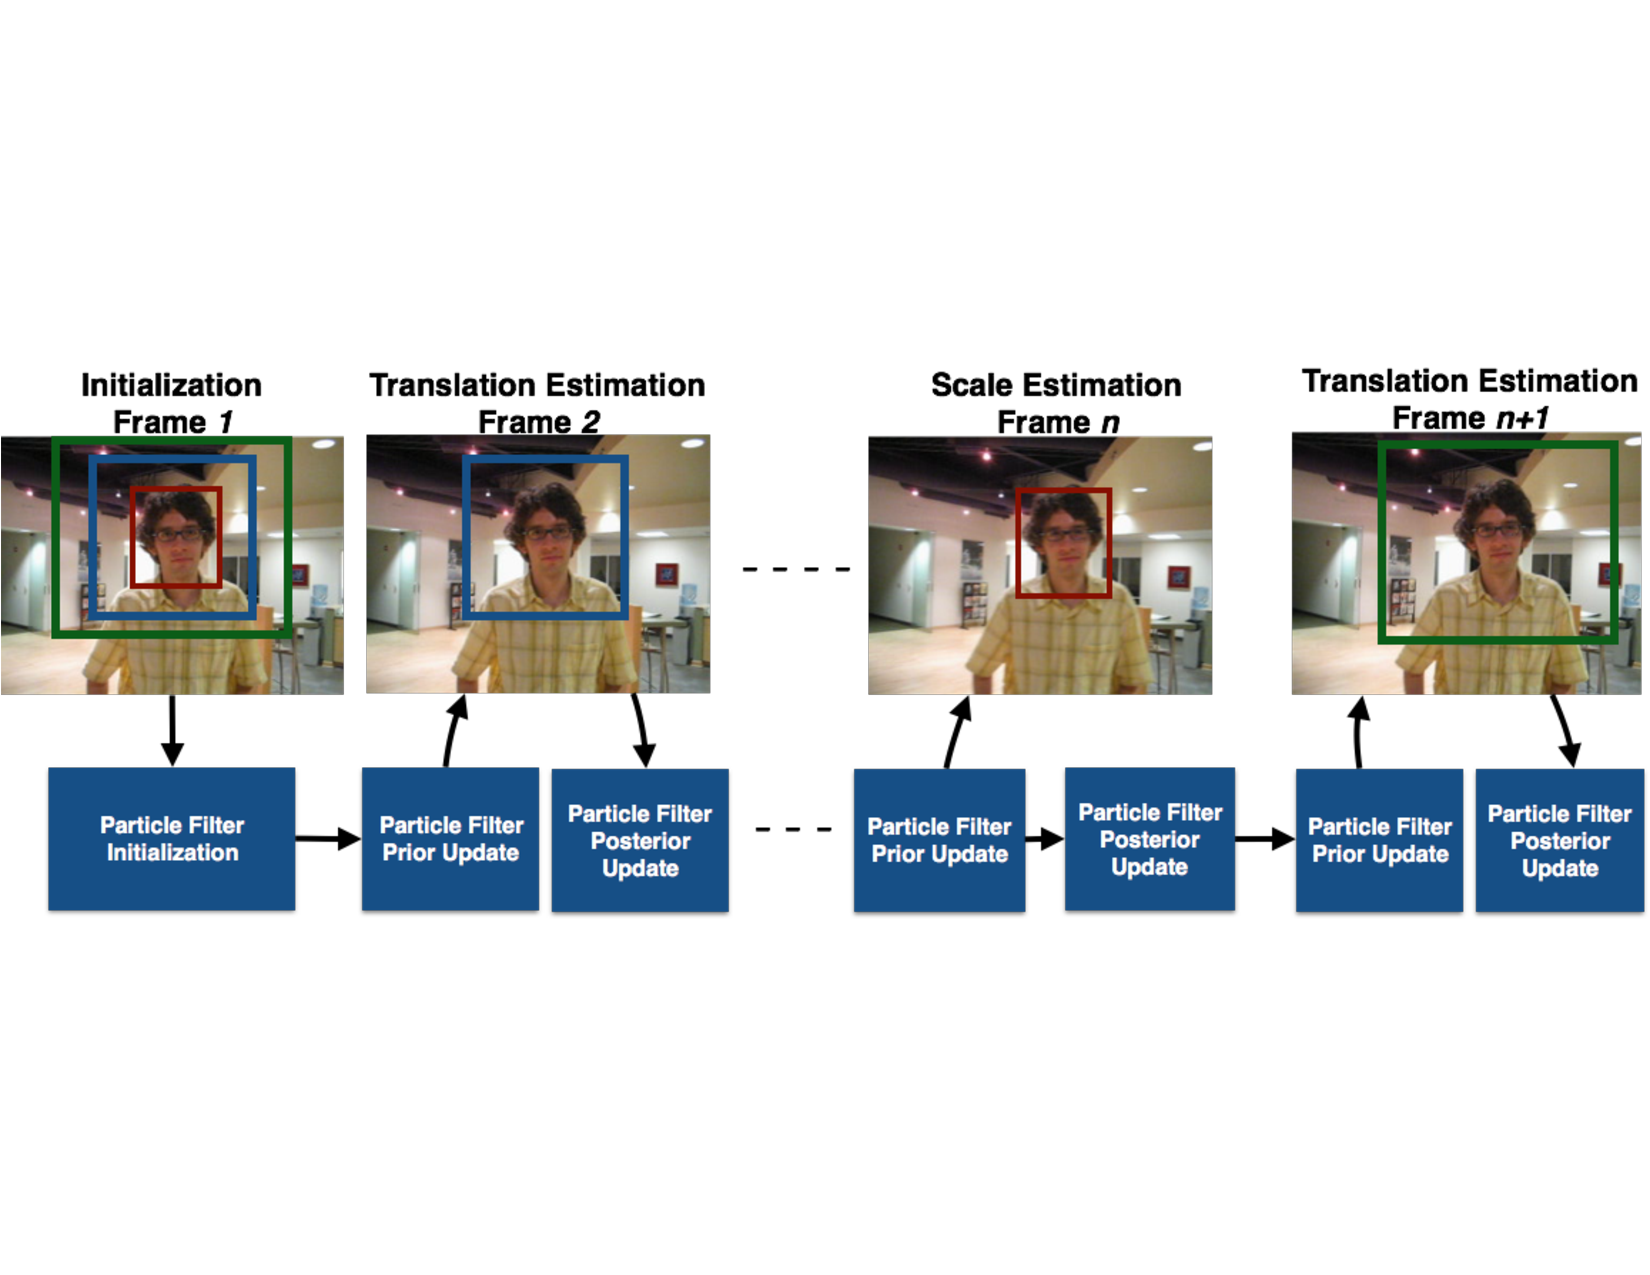
\includegraphics[width=\textwidth]{figures/Workflow_MKCF+PF.pdf}
\caption{The workflow of our Multiple KCF and Particle Filter based tracking method without the track re-detection module.}
\label{Workflow_figure}
\end{figure*}

Frequency domain correlation filter based trackers in the
tracking-by-detection paradigm has recently seen growing popularity
due to its superior computation and robustness to geometric and
photometric variations. The first correlation filter tracker proposed
by \cite{bolme2010visual} focused on learning and detection in the
frequency domain. The idea was to minimize the sum of squared error in
the frequency domain. Hence, the convolution in the original domain is
avoided, instead, element-wise multiplication is needed in the
frequency domain. This way, it achieved promising performance at 700
Hz. On the other hand, the MOSSE tracker failed in cases with rapidly
changing background as it learns the filter using a single template
and accommodates single channel features. Later on, the MOSSE tracker
was improved by using the circularly shifted background patches in an
efficient way by utilizing the theorem that Discrete Fourier Transform
of a circulant matrix gives us diagonalized circulant matrix
\cite{henriques2012exploiting,henriques2015high}. In the same work,
the authors integrated kernelization concept into the detection and
learning steps to improve tracking
accuracy. \cite{galoogahi2013multi,henriques2015high} extended the
correlation filter trackers with single channel features to
multi-channel features. They employed the color and shape features in
a simple framework by summing the correlation of the test and learned
feature channels elements. There a few major drawbacks of the
correlation filter trackers although they outperformed the other
discriminative trackers with superior computation. First, due to the
nature of correlation filters it is limited to a region of interest
which is typically 2-3 times larger than the target. Considering a
larger ROI not only increases the computational burden but also leads
to further spatial information loss with the fixed template size. For
this reason, its performance degrades in fast motion cases as the ROI
may not contain the target. Second, the correlation filter lacks scale
adaptation ability since it only estimates the translation of the
target. Later studies focused on improving the latter issue by
proposing scale candidates where each scale is assigned a confidence
by performing detection on the shrinked or enlarged the ROI
\cite{li2014scale,tang2015multi,bibi2015multi,ma2015long}. Another
group of studies employ the part-based correlation filter trackers to
better adapt to the scale changes
\cite{liu2015real,akin2016deformable}. The sensitivity to fast motion
is generally handled in the long-term target tracking framework where
track reinilization module is triggered when the target is lost
\cite{ma2015long,de2015board,li2016monocular}.

The contributions of this study are as follows.
\begin{itemize}
\item We build a highly efficient ($\geq300$ fps) scale adaptive multiple kernelized correlation filter based tracker that outperforms the original KCF implementation with fixed scale framework both in terms of accuracy and performance. The studies following the KCF improved the fixed scale framework by running detection on a number of candidate ROIs to figure out the new scale of the object after estimating the translation of the object. This approach adds additional complexity to the original KCF implementation and drags down the run-time performance from $300$ fps to less than $100$ fps.
\item We integrate the Particle Filter into the Multiple KCFs tracking as an additional filter that can avoid the drift due to one of the correlation filters we employ in our framework.
\item We propose a target re-detection module that can minimize the target loss due to the scale filter that learns the object model using only-object area. Also, the target re-detection step is required to handle severe occlusions, pose variations, illumination changes and fast motion.
\item Since our visual tracker mostly focuses on tracking objects from aerial moving platforms, we design a new robust target-to-camera distance estimation method. This way, a safe distance between the target and the camera-platform can be preserved.
\end{itemize}

% ---------------------------------------------------------
\section{Kernelized Correlation Filter Tracker}
\label{KCF}
% ---------------------------------------------------------
The Kernelized Correlation Filter tracker has recently been increasingly popular due to its operation at hundreds of frames per second with state-of-the-art tracking capabilities in
challenging cases. Its computational efficiency arises from its use of the discrete fourier transform of the circulant matrix and frequency domain element-wise operations knows hadamard product and division. The first example of frequency domain trackers is the Linear Correlation Filter tracker known as MOSSE tracker. It minimizes the ridge regression function
in the frequency domain using a single template with continous desired gaussian response. The KCF tracker, on the other hand, minimizes the regularized ridge regression function shown below. 
\begin{equation}
E(h) = \frac{1}{2}||y-\sum_{c=1}^{C}g*x_{c}||^{2} + \frac{\lambda}{2}\sum_{c=1}^{C}||h_{c}||^{2}
\label{eq:Closedform_RidgeReg}
\end{equation}
where $y$ represents the desired continous response whereas $h$ and $x_{c}$ represents the learned correlation filter and training template for the given channel. The $c$ parameter included in \cite{henriques2015high,galoogahi2013multi} makes it possible to integrate multi-channel features such as HoG and colour into the ridge regression function. The closed-form solution for the eq.~\ref{eq:Closedform_RidgeReg} can be obtained by setting the derivative of $E$ w.r.t $w$ to $0$. The solution in the primal domain can be formulated as
\begin{equation}
w = (X^{T}X+\lambda)^{-1}y
\label{eq:SpatialSolution}
\end{equation}
where $X$ and $\lambda$ represent the training samples and regularization term. The same cost function in the Fourier domain can be represented as
\begin{equation}
w = (X^{H}X+\lambda I)^{-1}X^{T}y
\label{eq:FourierSolution}
\end{equation}
More information on the spatial and fourier domain solutions can be found in \cite{henriques2015high}. The MOSSE tracker does not make use of $\lambda$ and only one training sample with desired response is used to update $w$. This framework does not include enough background information into the training framework with a single template. The application of the circulant matrix theorem into the eq.~\ref{eq:Closedform_RidgeReg} makes it possible to include many background patches at a similar computational complexity. A circulant matrix $C$ includes the circularly shifted patches of the positive training sample $x$ by the cylic shift operator $P$. By applying shifting operation to the base sample, we can generate the circulant matrix as
\begin{equation}
C = Px.
\label{eq:CirculantMatrixGeneration}
\end{equation}
The circulant matrix of a base sample $x$ can be interpreted as the rows of a training matrix $X$ where each row represents features of a training sample. Mathematically, this can be written as
\begin{equation}
X = C(x)
\label{eq:CIrculantMatrixTrainingData}
\end{equation}
In this form, eq.~\ref{eq:SpatialSolution} and~\ref{eq:FourierSolution} could prohibit us from implementing a high speed object tracking as we need to perform large number of element-wise division and multiplication operations. However, we know from \cite{gray2006toeplitz} that all circulant matrices are represented diagonally by the Fourier Transform regardless of the base sample $x$ as shown below.
\begin{equation}
X = Fdiag(\hat{x})F^{H}.
\label{eq:CirculantMatrixDFT}
\end{equation}
where $F$ denotes a constant Fourier Transform matrix and $x$ is the Discrete Fourier Transform of the base sample $x$. To simplify the cost function formulation in eq.~\ref{eq:FourierSolution} we multiply $X$ in eq.~\ref{eq:CirculantMatrixDFT} with $X^{H}$ yielding 
\begin{equation}
X^{H}X = Fdiag(\hat{x}^{*}\odot \hat{x})F^{H}.
\label{eq:SimplificationX} 
\end{equation}
Finally, the eq.~\ref{eq:SimplificationX} can used to formulate the solution vector in Fourier domain $\hat{w}$ as
\begin{equation}
\hat{w} = \dfrac{\hat{x}^{*}*\hat{y}}{\hat{x}^{*}*\hat{x}+\lambda}.
\label{eq:DiagonalizedPrimalSolution}
\end{equation}
For detailed documentation of the circulant matrix theorem based frequency domain solution can be found in \cite{henriques2012exploiting,henriques2015high}.

The above primal frequency domain solution can be called as Linear Correlation Filter which improves the MOSSE tracker by incorporating cyclic shifts and regularizer. To further improve the robustness to geometric and photographic variations, one can exploit non-linear regression function in the Correlation Filter framework \cite{henriques2015high}. The solution to the kernelized ridge regression function is shown below.
\begin{equation}
\alpha = y(K+\lambda I)^{-1}
\end{equation}
wjere $K$ and $\alpha$ represent the kernel matrix and corresponding dual space solution. \cite{henriques2015high} states that kernel matrices is circulant for datasets of circular cylic satisfying the following theorem. 
\begin{equation}
k(x,x^{'}) = k(Mx,Mx^{'})
\label{eq:KernelCirculantTheorem}
\end{equation}
where $M$ represents the permutation matrix. Some kernels satisfying the eq.~\ref{eq:KernelCirculantTheorem} are \textit{Gaussian}, \textit{Polynomial}, \textit{Intersection} and \textit{Hellinger} kernels. Similar to the diagonalization in the linear ridge regression solution in eq.~\ref{eq:DiagonalizedPrimalSolution}, the kernelized ridge regression can be made diagonal using the same circulant matrix theorem.  The diagonalized Fourier domain dual form solution can be expressed as
\begin{equation}
\hat{\alpha} = \hat{y}(\hat{k}^{xx}+\lambda)^{-1}
\label{eq:FourierDualDomainSolution}.
\end{equation}
where $\hat{k}^{xx}$ represents the first row of the Kernel matrix $K$ known as \textit{gram matrix}. In this study, we will only focus on application of the Gaussian Kernel to the Correlation Filters. We refer the readers to \cite{henriques2015high} for the detailed documentation of the application of other kernels to the Correlation Filters. For single channel features, the Gaussian kernelization is expressed as
\begin{equation}
k^{xx^{'}} = exp(-\dfrac{1}{\alpha^{2}}(||x||^{2}+||x^{'}||^{2}-2F^{-1}(\hat{x}^{*}\odot \hat{x}^{'})))
\label{eq:GaussianCorrelationSingleChannel}
\end{equation}
The first correlation filter based trackers used grayscale feature to learn the solution vector $w$, however, the multi-channel features such as HoG and Color were later exploited to improve tracking accuracy \cite{henriques2015high,galoogahi2013multi,tang2015multi,ma2015long,bibi2015multi}. The multi-channel feature integration into the Gaussian Kernelization function in eq.~\ref{eq:GaussianCorrelationSingleChannel} is achieved in a very straight-forward way by summing the correlation result in all the channels as
\begin{equation}
k^{xx^{'}} = exp(-\dfrac{1}{\alpha^{2}}(||x||^{2}+||x^{'}||^{2}-2F^{-1}(\sum^{C}_{c}\hat{x}_{c}^{*}\odot \hat{x}_{c}^{'}))).
\label{eq:GaussianCorrelationSingleChannel}
\end{equation}
Such non-linearization process does not increase the computational complexity of the linear multi-channel correlation filter dramatically as we only need to sum over the $n$ dimensional feature channels. Training shown in eq:~\ref{eq:FourierDualDomainSolution} gives us $\hat{a}$ learned in time step $t$. We can accumulate $\hat{a}$ over time to integrate more temporal information. This can be expressed as
\begin{equation}
\hat{a}_{t} = (1-\beta)\hat{a}_{t-1} + \beta\hat{a}_{t}. 
\end{equation}

Finally, detection step in multi-channel KCF framework is performed as
\begin{equation}
r(z) = F^{-1}(\hat{k}^{xz} \odot \hat{\alpha})
\end{equation}
where $r$ denotes the correlation response at all cylic shifts of the first row of the kernel matrix $K$. The peak point of the response function gives us the estimated translation of the object from time step $t$-$1$ to $t$.

\section{Multiple Kernelized Correlation Filter Based Tracking}
\label{sc:MKCF}
The KCF with Multi-channel features outperforms the other state-of-the-art object traking algorithms both in terms of run-time performance and tracking accuracy. However, it lack scale adaptation module or the naive scale adaptation method added into the KCF reduces the frames per second from $\geq300$ fps to less than $100$ fps. One straightforward method is to run detection on ROIs with different sizes determined by pre-defined scale ratios \cite{henriques2015high,tang2015multi,ma2015long,bibi2015multi,li2014scale}. All these method increases the computational complexity of tracking by running detection on a number of ROIs. Another scale update method in Correlation Filter framework was proposed by \cite{zhang2014fast}. It uses the MOSSE tracker to estimate translation of an object. The scale is updated in a naive way where the confidence map is used to determine the scale change between successive frames. For instance, their method assumes similar scale in between two consecutive frames given similar confidences. With this simple method, we do not need to run detection on different ROIs at a given frame and perform tracking at $\geq300$ fps. In this study, we propose the use of Multiple KCFs in an intuitive way to perform robust scale-adaptive tracking at more than $300$ fps. Our approach is inspired by \cite{ma2015long} where two KCFs are employed as translation and scale filters. It first estimates translation using the translation filter learned on \textit{target}$+$\textit{background} area. Then, the scale filter learned on the \textit{target} area is used to estimate new scale of the target at the estimated position. Application of translation and scale filter at each frame reduces run-time performance ($\leq50 fps$) as we need to run detection and training on both filters. Similarly, we learn three different correlation filters specializing on different aspects of tracking and addresses the weakness of each other, resulting in more robust tracking. We name these filters as \textit{target}+\textit{small background} translation filter ($R_{t}^{S}$), \textit{target-only} scale filter ($R_{s}$) and \textit{target}+\textit{large background} translation filter ($R_{t}^{L}$). Unlike \cite{ma2015long}, by running a single filter at each frame, we can achieve the targeted operation frame rate.
\begin{figure}[!t]
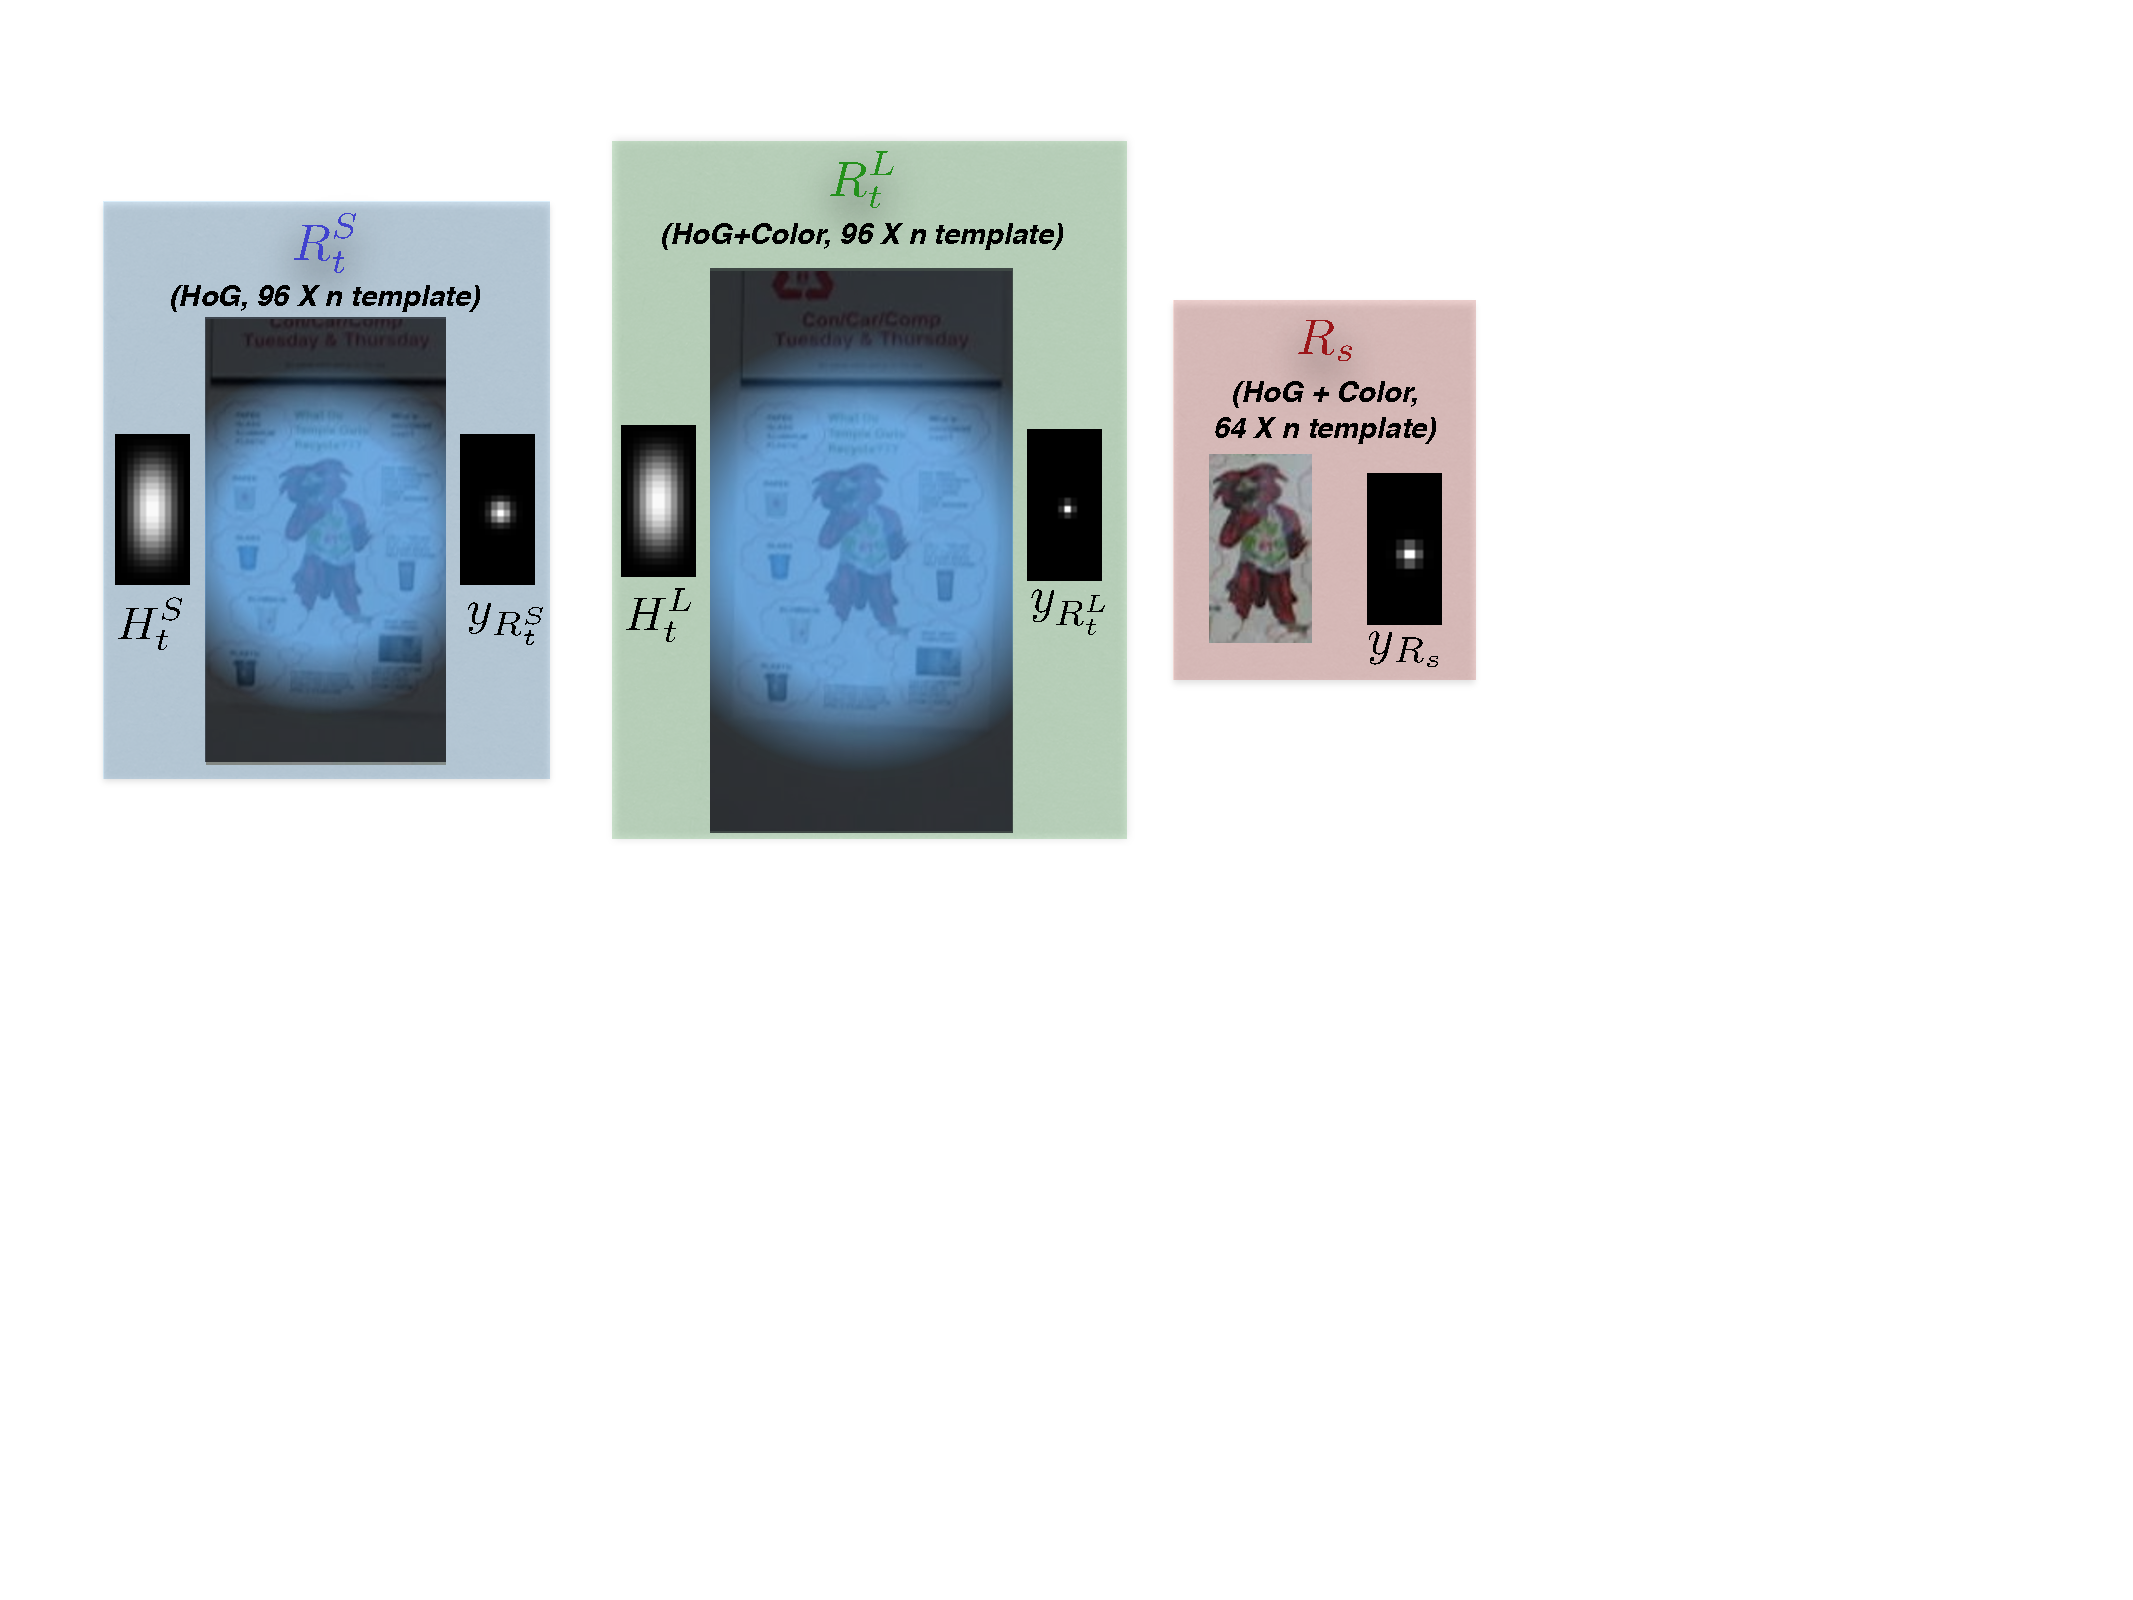
\includegraphics[width=0.5\textwidth]{figures/Filters_Details.pdf}
\caption{The three filters called as medium ROI translation filter, target ROI scale filter and large ROI translation filter are shown. Also, the hanning window and desired Gaussian response for each filter are displayed.}
\label{fig:Filters}
\end{figure}

\section{Particle Filter}
\label{sc:PF}

\section{Track Re-initilization via Re-detection}
\label{sc:Re-initialization}

\section{Geometry Estimation between Target and Drone}
\label{sc:Geometry}

\section{Experiments}
\label{sc:Experiments}

\section{Conclusion}
\label{sc:Conclusion}
%--------------
%\section*{Acknowledgements}
%put stuff here for the accepted , but not the ICCV version


\small
\bibliographystyle{ieee}
\bibliography{draft}

\end{document}
